\postextual
% ----------------------------------------------------------

% ----------------------------------------------------------
% Referências bibliográficas
% ----------------------------------------------------------
%\bibliography{references} %if using bibtex
\printbibliography %if using biblatex

% ----------------------------------------------------------
% Glossário
% ----------------------------------------------------------
%
% Consulte o manual da classe abntex2 para orientações sobre o glossário.
%
%\glossary

% ----------------------------------------------------------
% Apêndices
% ----------------------------------------------------------

% ---
% Inicia os apêndices
% ---
%\begin{apendicesenv}

% Imprime uma página indicando o início dos apêndices
%\partapendices

%\end{apendicesenv}
% ---


% ----------------------------------------------------------
% Anexos
% ----------------------------------------------------------

% ---
% Inicia os anexos
% ---
\begin{anexosenv}

% Imprime uma página indicando o início dos anexos
\partanexos
    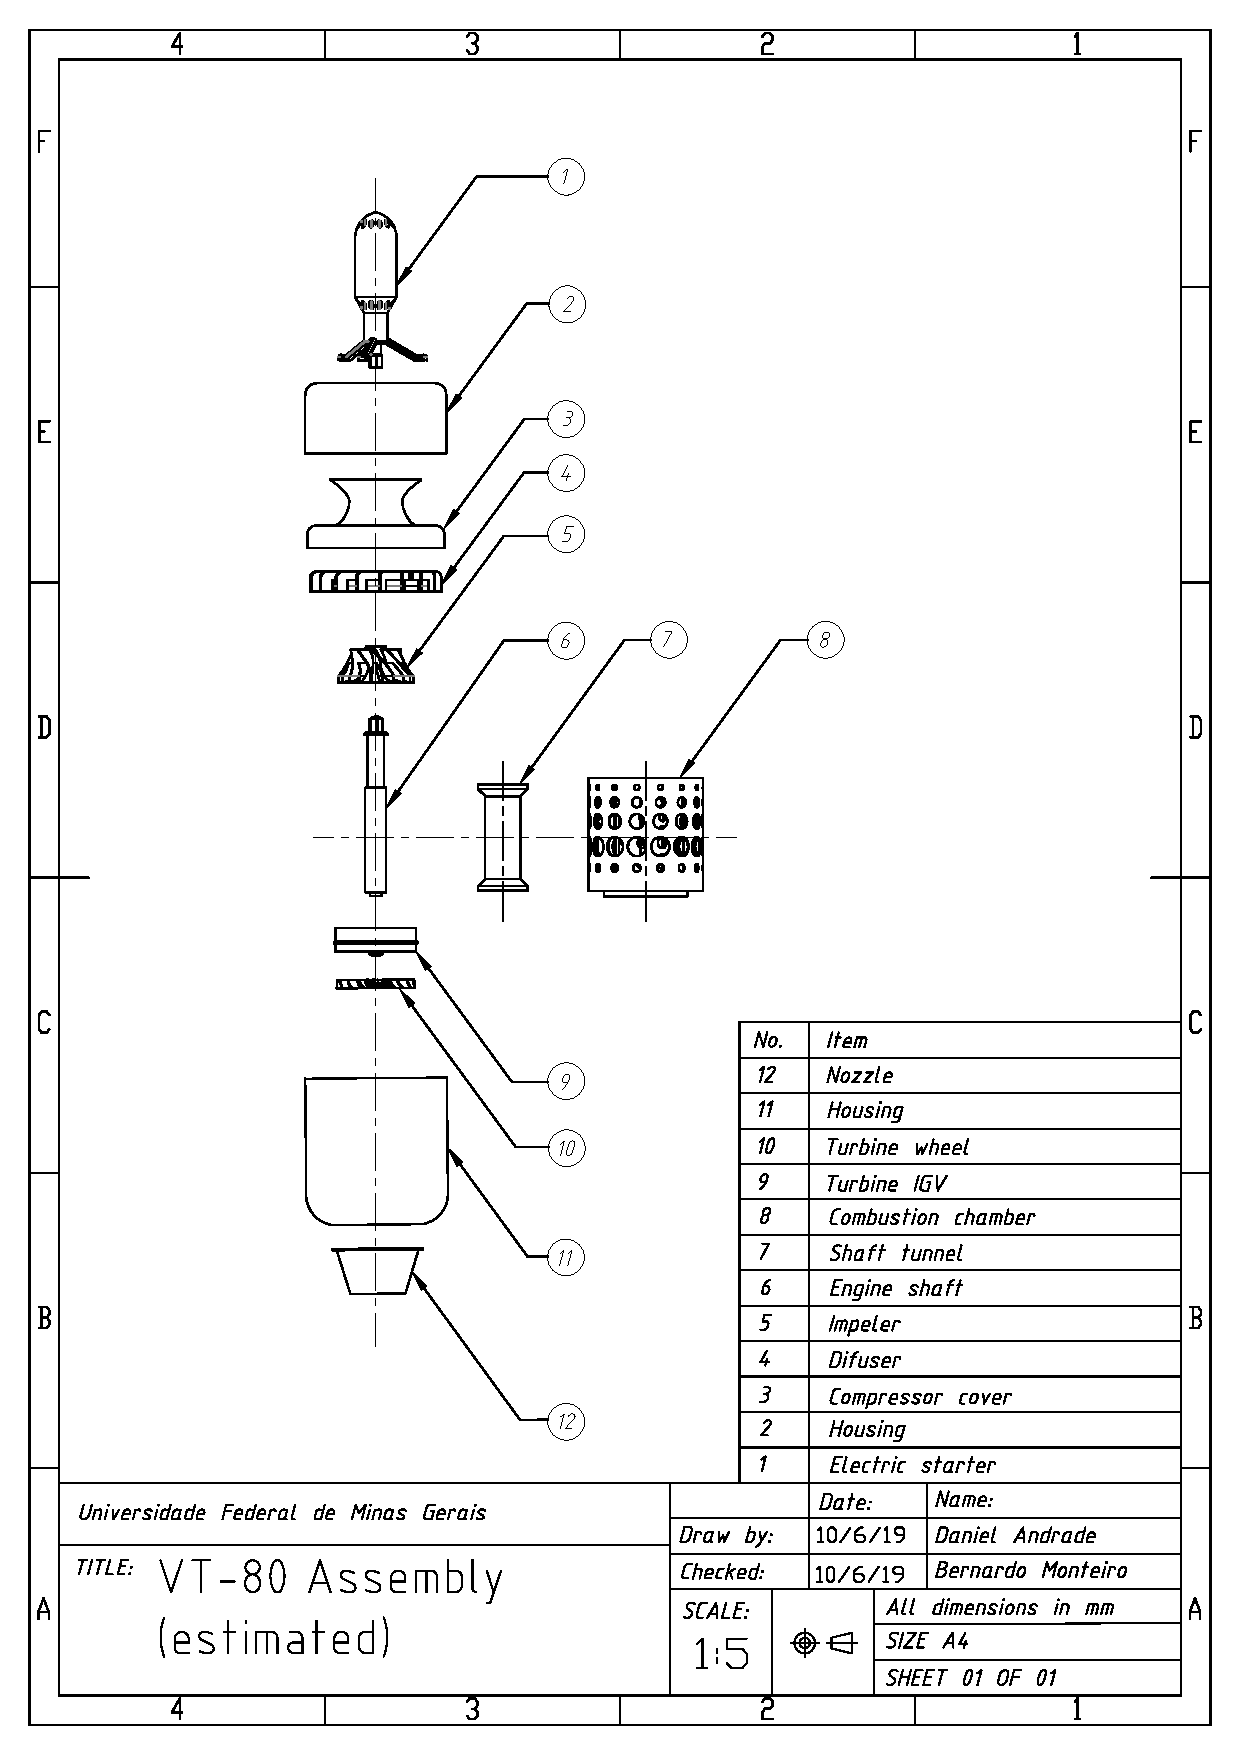
\includepdf[addtolist={1,figure,VT-80 assembly,dwg:assembly}]{drawings/VT-80_Assembly}
    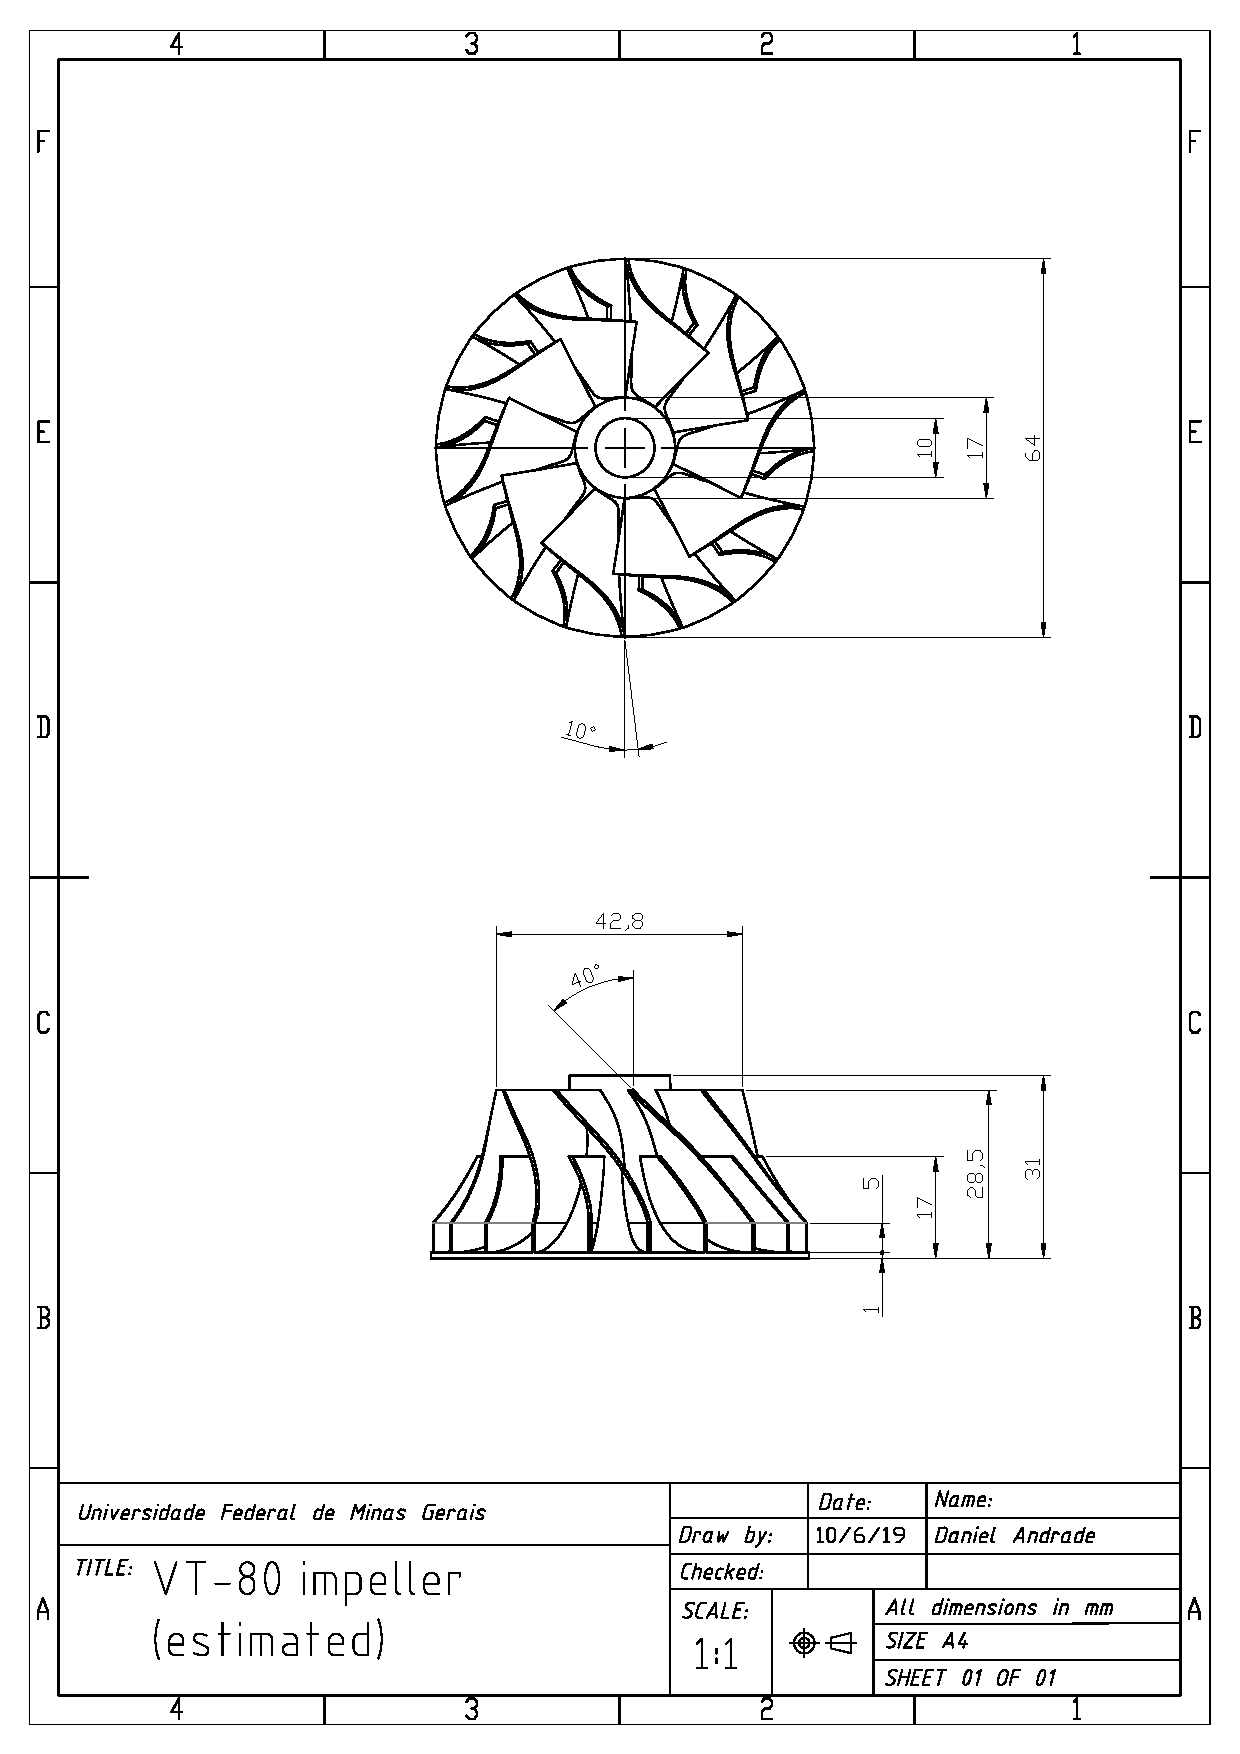
\includepdf[addtolist={1,figure,VT-80 impeller,dwg:impeller}]{drawings/VT-80_Impeller}
    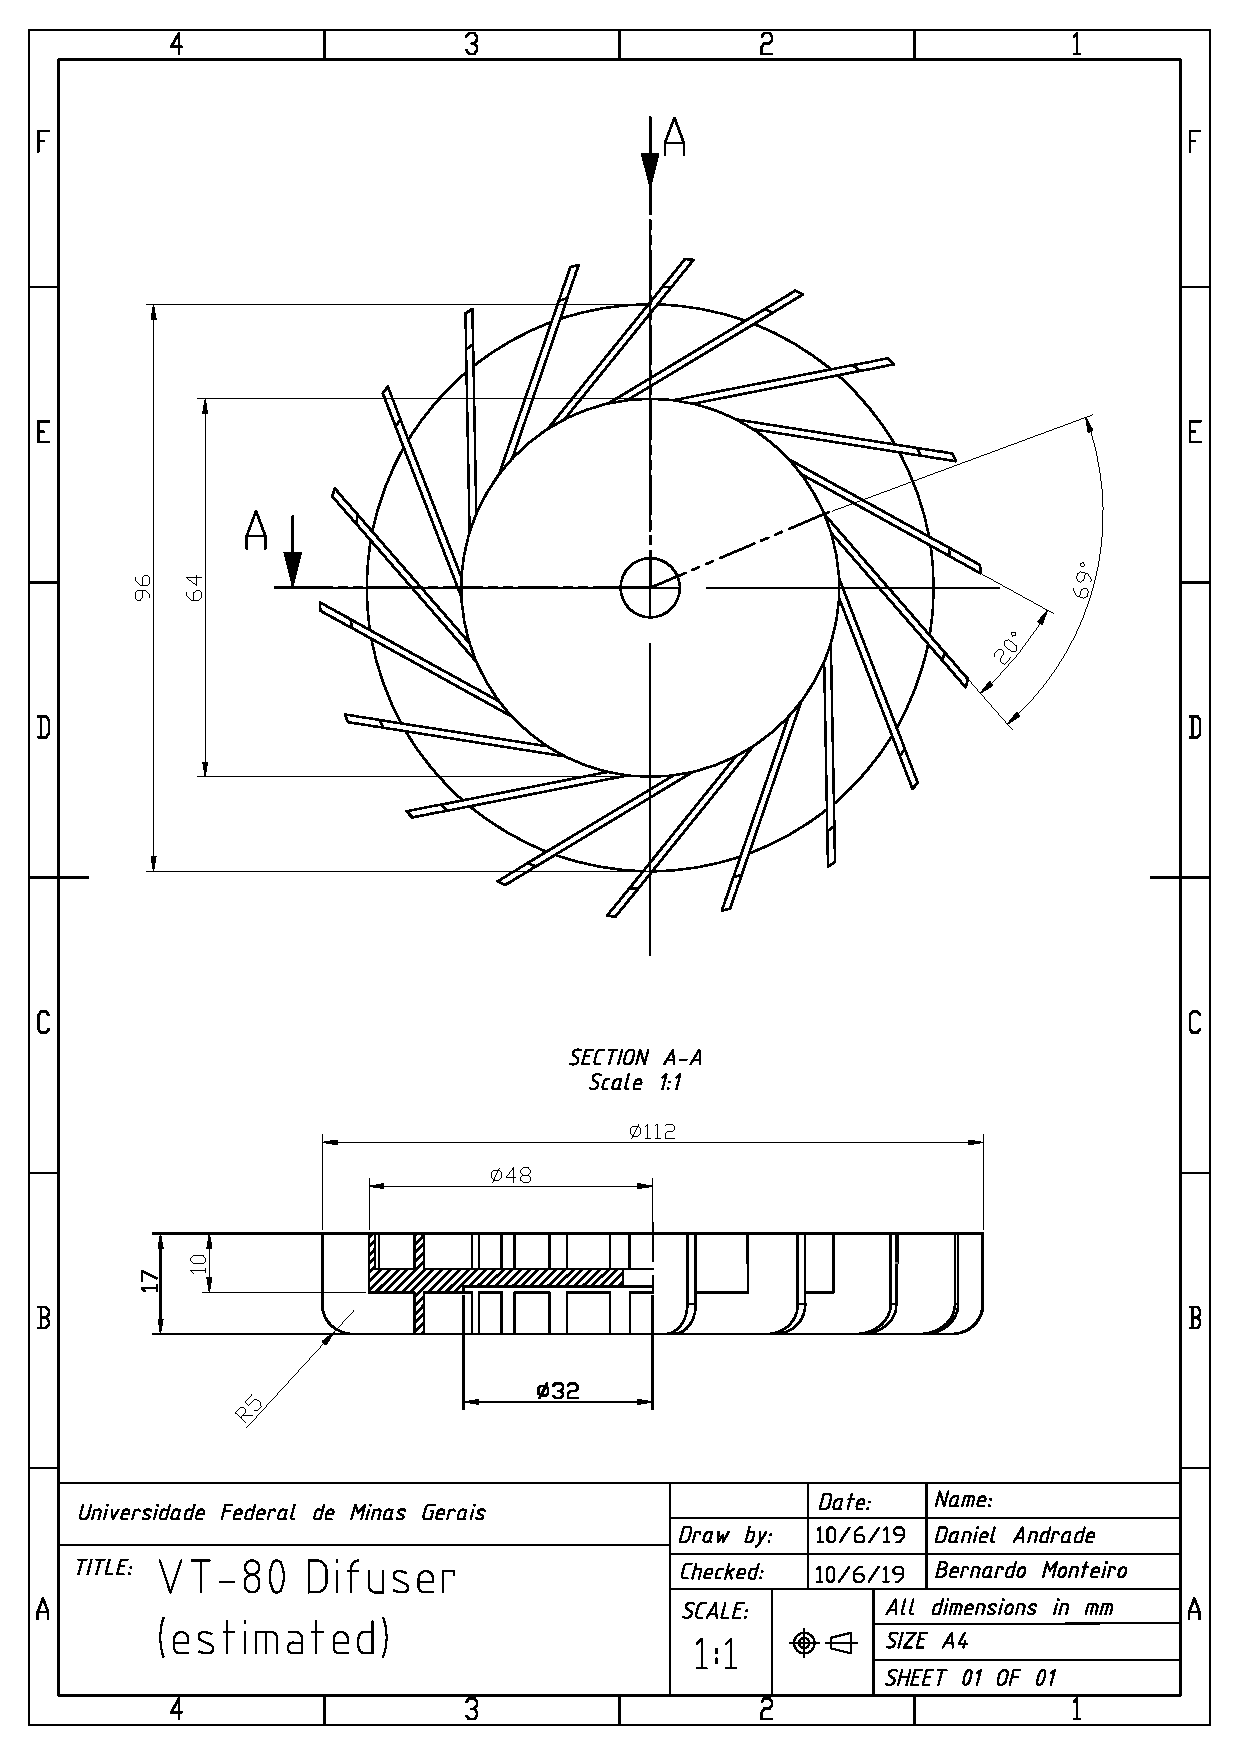
\includepdf[addtolist={1,figure,VT-80 difuser,dwg:difuser}]{drawings/VT-80_Difuser}
    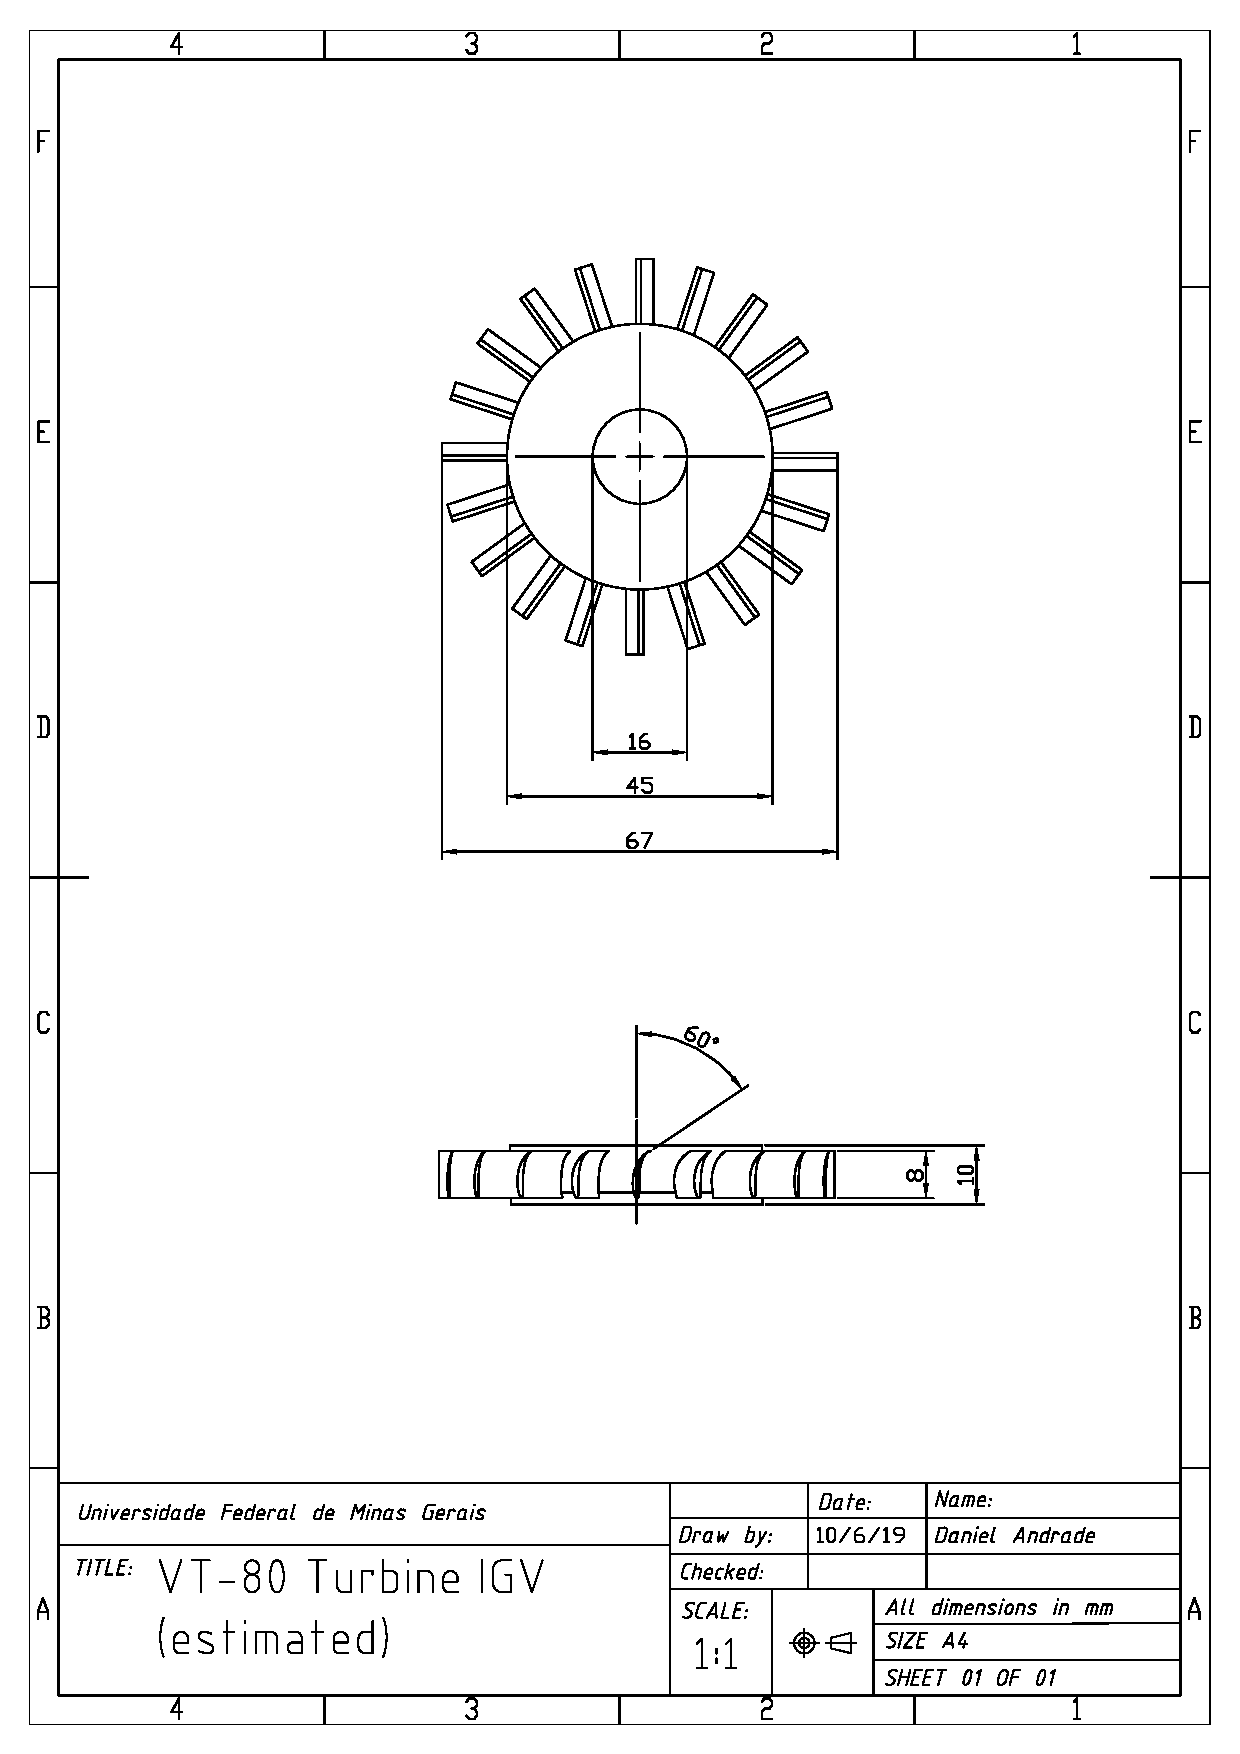
\includepdf[addtolist={1,figure,VT-80 turbine inlet guide vanes,dwg:igv}]{drawings/VT-80_Turbine_IGV}
    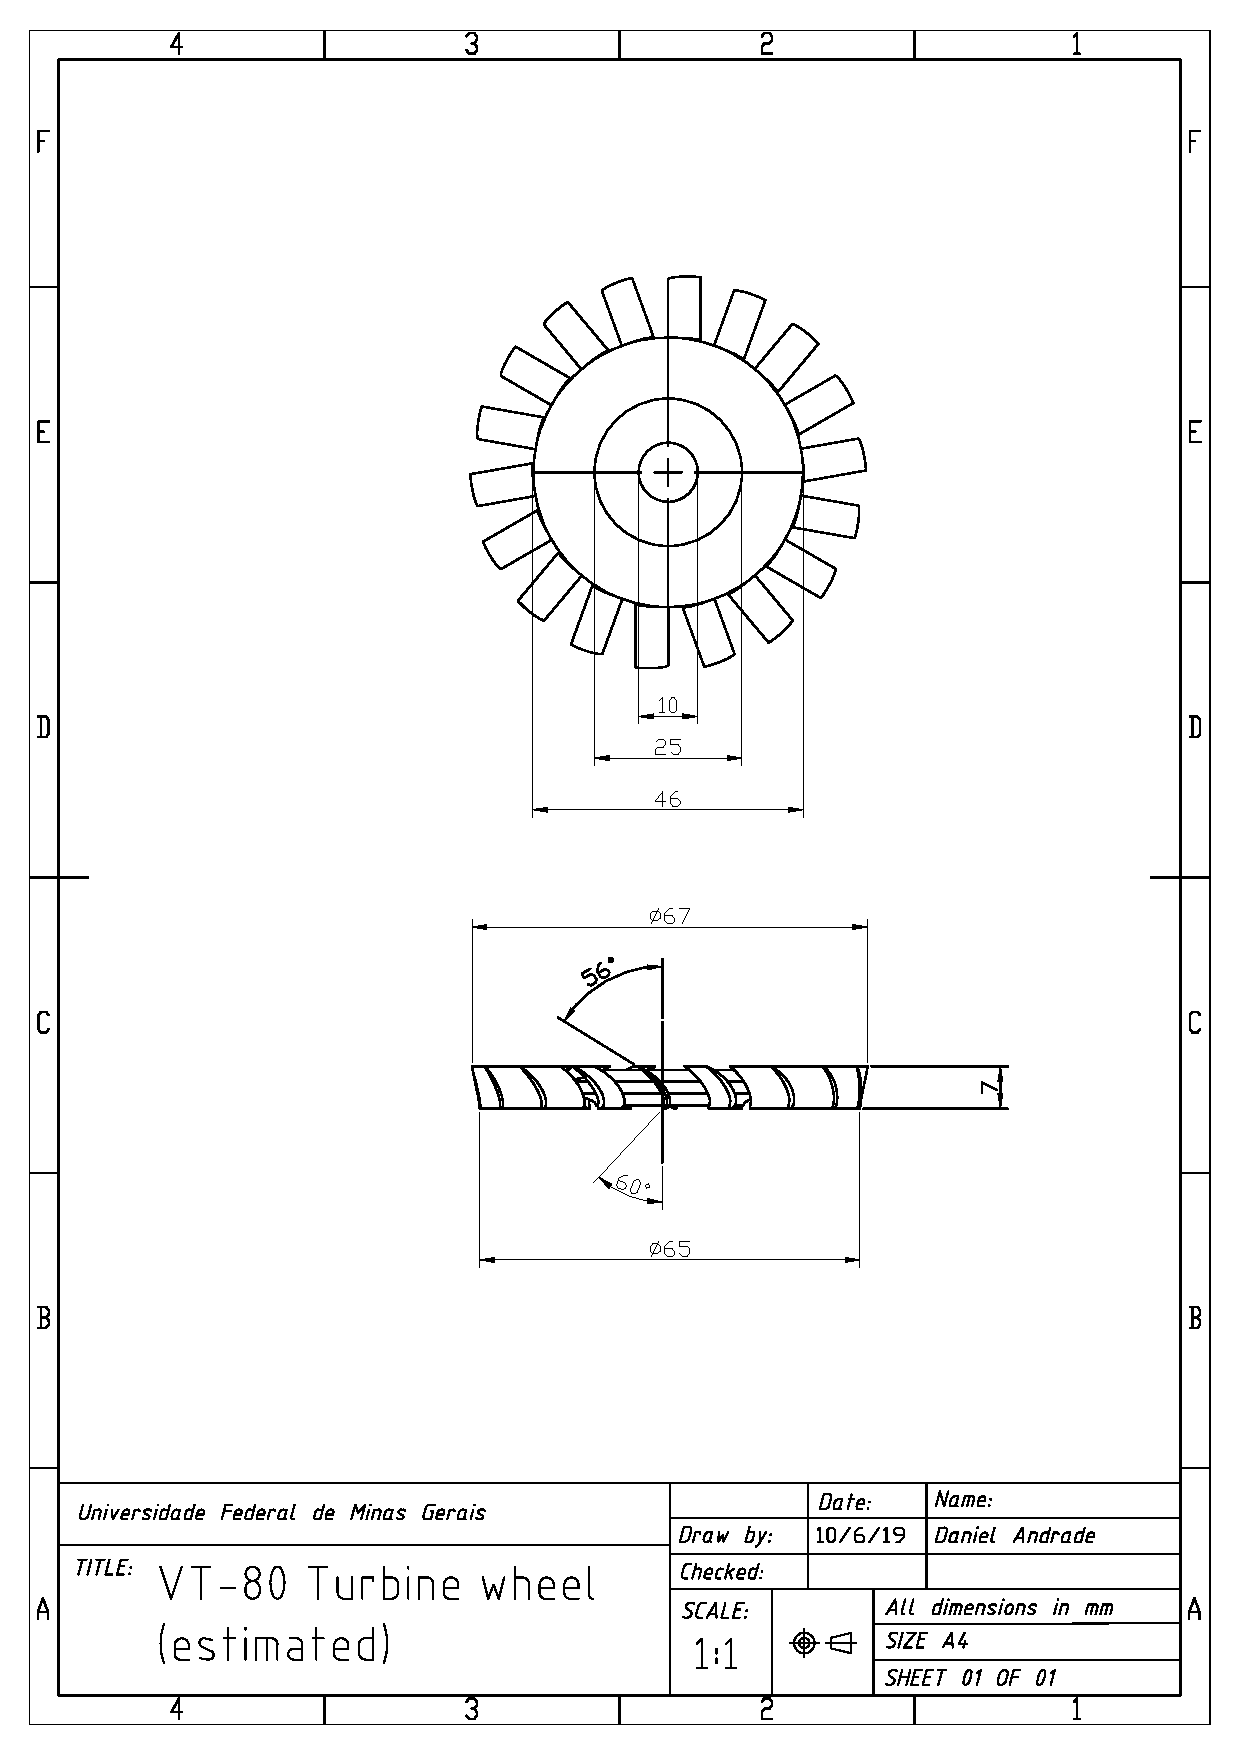
\includepdf[addtolist={1,figure,VT-80 turbine wheel,dwg:turbine}]{drawings/VT-80_Turbine_wheel}

\end{anexosenv}

%---------------------------------------------------------------------
% INDICE REMISSIVO
%---------------------------------------------------------------------
%\phantompart
%\printindex
%---------------------------------------------------------------------
